\documentclass[a4paper,12pt]{article}
\usepackage{unifrsr}
\usepackage{hyperref}
\usepackage{minted}
\usepackage{amsmath}

\begin{document}
\seminartitle{Human Smart Cities Seminar} % The title of the seminar

\title{
   Finding Files and Experts in Your Field: \\ 
   \large How Solr Can Help} % The title of your project


\author{
   Elias Wipfli (13-123-922) 
   \thanks{\email{elias.wipfli@students.unibe.ch}, University of Bern}
   \and
   Julius Oeftiger (16-127-532) 
   \thanks{\email{julius.oeftiger@students.unibe.ch}, University of Bern}
   \and
   Brian Schweigler (16-102-071)
   \thanks{\email{brian.schweigler@students.unibe.ch}, University of Bern}
}

\supervisor{Prof. Edy Portmann} % Name of the supervisor

\assistant{Minh Tue Nguyen \and Moreno Colombo \and Jhonny Pincay} %Name of the assistant(s)

\date{31 December 2021} % Note: if this is left out, today's date will be used, this is the submission date!

\maketitle

\begin{abstract}

TODO Abstract


\keywords{Seminar report, Human-IST Research Institute, Human Smart Cities, Smart Governance, Solr,}



\end{abstract}

\textbf{Public Git Repository:} \href{https://github.com/Brian6330/Human\_Smart\_Cities}{https://github.com/Brian6330/Human\_Smart\_Cities}.

\tableofcontents
\newpage

\section{Introduction}
Cities are adopting Information and Communication Technologies (ICT) more and more into their services.
Thus, the need to address challenges in such Human Smart Cities keeps rising.
As the citizens are the main drivers of change, they must be included to best handle these challenges \cite{oliveira_smart_2015}.

One such challenge that must be addressed is the dispersion of information among different systems and applications.
Most importantly, this information must be found within a short time-frame.
If parts of the retrieved data is unclear, talking to an expert might be of importance.
This leads to the follow-up issue of determining who is likely to be an expert in a specific field.

The Research Questions focused on are:
\begin{enumerate}
\item Given multiple text files, how can their contents be searched to return the best fitting ones?  
\item How can a list of experts be extracted from the submitted text files?  
\item The submitting user of a given text file, must not necessarily be the user who wrote it. 
      How can this be considered when determining the expert list?
\end{enumerate}

The remainder of this project report is structured as follows: 
the required background to understand certain terminology and methods used is explained in chapter 2, 
related works are mentioned in chapter 3
Solr is talked about in length in chapter 4,
the methodology used is thoroughly explained in chapter 5, 
in chapter 6 the evaluation procedure is described, 
in chapter 7 the project results will be presented 
and in chapter 8 the report will be concluded while also providing a short outlook on possible extensions to the work.


\section{Theory} % Chapter that relates the project to and talks about Human Smart Cities (re: Presentation feedback)
- What did we need to understand that readers may need to understand to?


- TODO Insert content for this (introductory) section; do we have more than one subsection? (Stemming)

\subsection{Determining Experts}
Who is an expert in a given topic?
To determine this, the extracted text content is tokenized with the Natural Language Toolkit (NLTK) \cite{nltk}.
There are a lot of so-called "stop-words" in the English language \cite{rajaraman_mining_2014}, that must be filtered out, as they are not relevant to determine who is an expert in a given field. 
Examples of such stop-words that are filtered out: 'the', 'and', 'from'. 

After this step, a list of the most frequent terms is returned. 
It is possible to limit the number of terms returned in the code; the current limit of returned terms is 50.
To determine the score of the term, the earlier the term is within the expert's list, the more knowledgeable the expert is in regard to the chosen term. 
This can be expressed as follows: 

\begin{center}
    $ \text{Score} = \frac{(\text{Cut-Off} - \text{index})}{\text{Cut-Off}}$ 
\end{center}

To better illustrate this, we will look at an example where the $ \text{Cut-Off} = 50 $:
\begin{center}
Expert A has [snow] at index 6.			$\rightarrow$ 	$\text{Score} = (50 - 6) / 50 = 0.88$


Expert B has [snow] at index 4.			$\rightarrow$ 	$\text{Score} = (50 - 4) / 50 = 0.92$

\end{center}

Thus, Expert B would be more knowledgeable in regard to 'snow' than Expert A in our scoring system.

\newpage
\section{Related work}

\subsection{Building a Hierarchical, Granular Knowledge Cube}
This paper \cite{Denzler2015BuildingAH} proposes to build a knowledge cube with a hierarchical structure, where every lower level gets more granular and the uppermost layer is the coarsest one. 
A knowledge cube is composed of multiple granules on the multiple levels of the cube. 
These granules are composed of concepts, which have relations to other concepts on the same granular level or on others.
Similar like the relations in regard to the concepts, the granules have dependencies to upper level granules. Concepts are atomic information that are extracted from content with data-mining, which are then grouped together with related concepts into a granule. 
The advantage of this knowledge cube is, that a domain may stretch vertically as well as horizontally, and through this it may reveal structural regularities or irregularities. 
To fill the cube with knowledge, an automatically or semi-automatically approach should be chosen. 
The proposed cube should have three layers, where the first layer is for storing, the second for the representation of the knowledge and in the last layer is the structure of the knowledge.


\subsection{An Expert/Expert-Locating System Based on Automatic Representation of Semantic Structure}
This paper \cite{EEL} proposes the idea of finding an expert with the use of input documents, which are then analyzed to create the corresponding expert system. 
The process first extracts the text of the documents and removes stop words or punctuation marks, then it changes the plural words to singular and isolates compound words. 
By using the semantic structure analysis, which relies on singular value decomposition, the resulting EEL-system is better than standard keyword matching, because it also takes into consideration documents, which are related. 
Sadly, the system has a problem with negation and does not know how to deal with it.


\section{Solr}
Before we could start with our proof of concept, we needed an already existing framework which satisfies our demands.
The found framework is Apache Solr\cite{Solr}.
Solr\cite{Solr} is an open-source search application built on Apache Lucene, which can handle for example PDFs and allows a full-text search or indexing on them. 
If Solr searches a document, it performs the following operations:

\begin{enumerate}
    \item Indexing 
    \item Querying
    \item Mapping
    \item Ranking
\end{enumerate}

\subsection{Solr Methodology} % Could be renamed
First, the searched document is converted into machine-readable form, which can be done as explained later by simply extracting all relevant information from the document. 
The query terms has to be specified by the user, which is then used in the next operation. 
In this third operation, the now machine-readable document is searched for a specified term or image. 
At the end, a ranking is done depending on the search results. As can be seen, we will later use this ranking and the already existing search feature of Solr.



To start a Solr server, one could simply follow the \href{https://solr.apache.org/guide/8_11/solr-tutorial.html}{Solr tutorial}. 
First, the current Solr executable has to be downloaded and installed. 
Then the Solr server can simply be started by the following command: 

\begin{minted}{bash}
./bin/solr start -e cloud
\end{minted}

This command starts the Solr server in cloud mode and the user has to enter further information like for example the port where the application and how many nodes should be run. 
At the end, there is also a choice which configuration should be used. 
Instead of the default configuration, the $\textbf{sample\_techproducts\_configs}$ is used, because the additional request handlers of this provided configuration can then be used. 
What should be noted is, that the same command above can be used on a Windows computer, but if the $\textbf{solr.cmd}$ is used instead, then there may arise the problem on how to close the started Solr server again. 
The solution would be to find with the command line the corresponding $\textbf{pid}$ of the server and kill it directly, because the regular Solr command to stop a server would not find this server.


Because these commands have to be made at the beginning of every start of the Solr server, and possible modification or restart, it is clear that this approach is error-prone. 
We asked ourselves if there is a method where we simply can start one single command, which sets the Solr server up without the need of user interaction.
The technology which answers this demand is Docker (section \ref{sec:docker}).


\subsection{Solr - How It Works}
Solr is configured via a schema file. 
It tells Solr about the contents of documents it will be indexing. 
The schema file used is also $\textbf{sample\_techproducts\_configs}$, as mentioned prior, as it has a request handler defined for extracting text from documents.
Text is extracted via Apache Tika, a toolkit that "detects and extracts metadata and text from [...] different file types (such as PPT, XLS, and PDF)" \cite{apache_tika}. 

Solr uses its own data structure to save its content.
It consists of a document containing multiple fields, each with a name and its content:

\begin{itemize}
    \item id: A unique ID (UUID), that is created for each document upon upload.
    \item last\_modified: The date the PDF was last modified, according to its metadata.
    \item content\_type: What type of content the document is (e.g. 'application/pdf')
    \item author: The author of the PDF, according to its metadata.
    \item author\_s: Secondary author field from the PDF, according to its metadata. Does not always exist.
    \item content: The by Tika extracted text, includes special symbols and line breaks (e.g. \textbackslash n)
    \item title: The title of the PDF, according to its metadata.
    \item links: Links found in the PDF file, be it to external webpages or interal files and images used.
    \item subject: Often empty, extracted from the PDF metadata.
    \item: \_version\_: An internal field used by Solr.
\end{itemize}


\subsection{Solr Request handlers}
"A request handler process request coming to Solr" \cite{apache_solr_reference_guide_requesthandlers}. 
The default request handler is 'select', which takes query parameters to search for terms.
Another important one for this project is /update and /update/extract. 
Both can be used in conjunction with binary data to generate a HTTP POST request, allowing the pushing of new items to the Solr server.
If we are dealing with a PDF or similar and want its content, only update/extract allows the extraction of the text content with Apache Tika.


\subsection{PySolr}
\href{https://pypi.org/project/pysolr/}{PySolr} is a simple client for Apache Solr based on the programming language Python. 
It allows the user to connect to an already running Solr server and query requests from the server with so-called request handlers or upload files to it. 
Like most open source packages, the documentation is rather sparse. 
PySolr facilitated the communication between the created scripts and the running Solr server.


\section{Methodology} % What we are doing, how we are doing it
Coded in python.

How is GUI created?

...

...


\subsection{Docker}
\label{sec:docker}
\href{https://www.docker.com/}{Docker}\cite{Docker} is a software which allows the user to deploy another software in a virtualized environment on the operating system. 
The deployed software is run in a so-called "container", which is like a small virtual machine with a standardized environment, where the dependencies are provided. 
This allows the user to run software on multiple platforms without the need to adjust  the software for all possible operating systems, and instead the user just has to make sure that Docker runs. 
Different from a regular virtual machine, a container does not have a high overhead and can use the underlying resources of the system better, which leads to a higher efficiency. 
Every deployed software is a single instance of an application, so Docker is very useful for scaling demands of an application, because to satisfy these demands, the number of instances of the application can be increased and decreased as needed.


A Docker image is a set of instructions of how the container is built and are comparable to snapshots for a virtual machine. 
The image contains the application code, libraries, dependencies and other files which the software would need to run the application. Most images are stored on a so-called registry, most of them on the docker registry. 
If an image changed, then the difference from the old to the new image is stored on the registry, so it is layer based. 
One could generate a custom image by setting up a Dockerfile, which is then executed, and the resulting image can be pushed to a registry. Luckily for our purpose to use Solr, there is an existing image on the docker registry. 


If we would simply use the Solr image with normal commands, then the user would have to not only start the container, but also executing a command to create a core for Solr, then another command to create the collection. 
This is rather troublesome, because if one command is forgotten, the whole application won't work correctly. 
Docker Compose would be a method to run multiple containers at once, or in other words to start different container sequentially which would then execute the needed commands.
There is an example of docker compose for \href{https://github.com/docker-solr/docker-solr-examples/blob/master/docker-compose/docker-compose.yml}{Solr} which we were able to use.
First, it started a stand-alone Solr server and uses zookeeper, which connects the different containers in a network together. 
But sadly, this example is incomplete, as we had to append the commands for creating a core and collection in an additional container. 
There is also a command where a directory can be selected, from which the content is uploaded to the running Solr server.


This customized Solr application can now be started, restarted and closed pretty easily in our chosen IDE. 
But we had to drop this approach, because the documentation was insufficient to help us how we could change the schematics of the core for uploading PDF files. 
This special schematics was needed, so that we could use PySolr and extract the text from an uploaded PDF file, but it isn't available if Solr is started with Docker. 
Even though we had to discard Docker for our proof of concept, we would still advise the use of it in further human smart cities project, as explained above it removes the need to adjust a software on multiple platforms.

\subsection{Data Source}
For this project, the data used were PDFs created by "EnviDat: das Umwelt-Datenportal". 
It is one of the organizations that have open data on \href{https://opendata.swiss}{https://opendata.swiss}.
The PDFs used needed to be in English, have properly encoded text (so it can be extracted by Tika) and contain more than just images or diagrams.

In total, 18 PDF files were used with 6 different authors. 
Those with an empty author field were ignored for the expert list, but can still be perused when searching for keywords with Solr.
While text analysis could have been done to determine authors from the first page of the PDF files or even from looking at the text formatting, it was decided that this would not be done for the proof-of-concept. 
Nonetheless, it is a valid extension and might also help to differ between text uploaders and text authors.


\subsection{Expert List Caveats}
Despite its simplicity, the scoring method used to determine experts, coupled with our Solr-based approach, leads to a few caveats:
\begin{itemize}
    \item Snow $\neq$ Snowing $\neq$ Snowfall $\rightarrow$ No stemming applied.
    \item Keywords belonging to one domain are not grouped as they should be. 
        
        e.g.\ (Permafrost; Snow; Rain) $\in$ “Glaciology” or "Climatology".
    
    \item Scoring alternatives may be better suited.
    \item Assumption uploader = author $\rightarrow$ PDF Metadata not reliable.
\end{itemize}

While Solr has some stemming in regard to searches, most of them need pre-defined rules.
Grouping by domain would also require defining what terms belong together (e.g. 'rain' and 'precipitation').
Regarding scoring, alternatives may be better suited for certain tasks, but it can always depend on the texts that are analyzed.
Lastly, the assumption that the uploader is the author could be fixed with a pop-up when uploading a PDF, where one could correct or fill in the required information. 

\section{Evaluation} % How we are evaluating our work.
Is the correct expert returned as first or second recommendation?
Going off of the assumption, that a user will only look at the first two experts recommended, to turn to them for further information, a correct recommendation is defined as when the first or second expert is an actual expert.

\subsection{Metric}
The metrics that were used are precision and recall. 
Let $AP$ be the actual positives, $AN$ the actual negatives, $TP$ and $FP$ true
and false positives, and $TN$ and $FN$ true and false negatives. Then:

\begin{center}
    $\text{Precision} = \frac{TP}{TP + FP} $
\end{center}

\begin{center}
    $\text{Recall} = \frac{TP}{AP} $
\end{center}

Precision can be understood as how many selected items are relevant, 
while recall can be understood as how many relevant items are selected.


\subsection{Test Set}
The test set used is made up of 18 files, with 170 unique terms, attributed to 6 authors.
This test set was created manually, by going through the papers and entering what we deem to be the relevant terms.
Furthermore, it is supplemented by 5 - 200 automatically determined terms, taken from the most frequent terms for each author. 


\textbf{This test set has several biases: }

\begin{itemize}
    \item The 170 manually determined “test” terms have a large impact on the test set.
    \item Randomly generated English words, resulted only in true negatives and were not usable.
    \item No true negatives – terms either in one or both of the sets.
\end{itemize}

The impact of the test set can be minimized by increasing the "cut-off" value for the automatically determined words, so they outnumber the manually determined keywords.
If the test set looked at more PDF files, randomly generated keywords may have been a valid approach, but with the current 18 files, it is simply not sensible to use only automatically generated English words.
Lastly, even if our test has no true negatives, the return data can still paint a picture of how useful the output is.


\section {Result} % The results of our work, as well as the evaluation
What happened?

What can we show as a result? (Screenshots? Walk-through of an example?)

What is new to our approach?

...

...

\subsection{Evaluation Result}
The returned experts were compared to the test-set for cut-off/threshold values of 5, 10, 15, 20, 35, 50, 100, 200 most frequent words per author. 
Tests were run five times for the same configuration, with each configuration taking 100 random terms.
These five runs were then averaged to receive a more stable result, with precision and recall scores falling within [0,1].

\begin{figure}[h]
    \begin{center}
        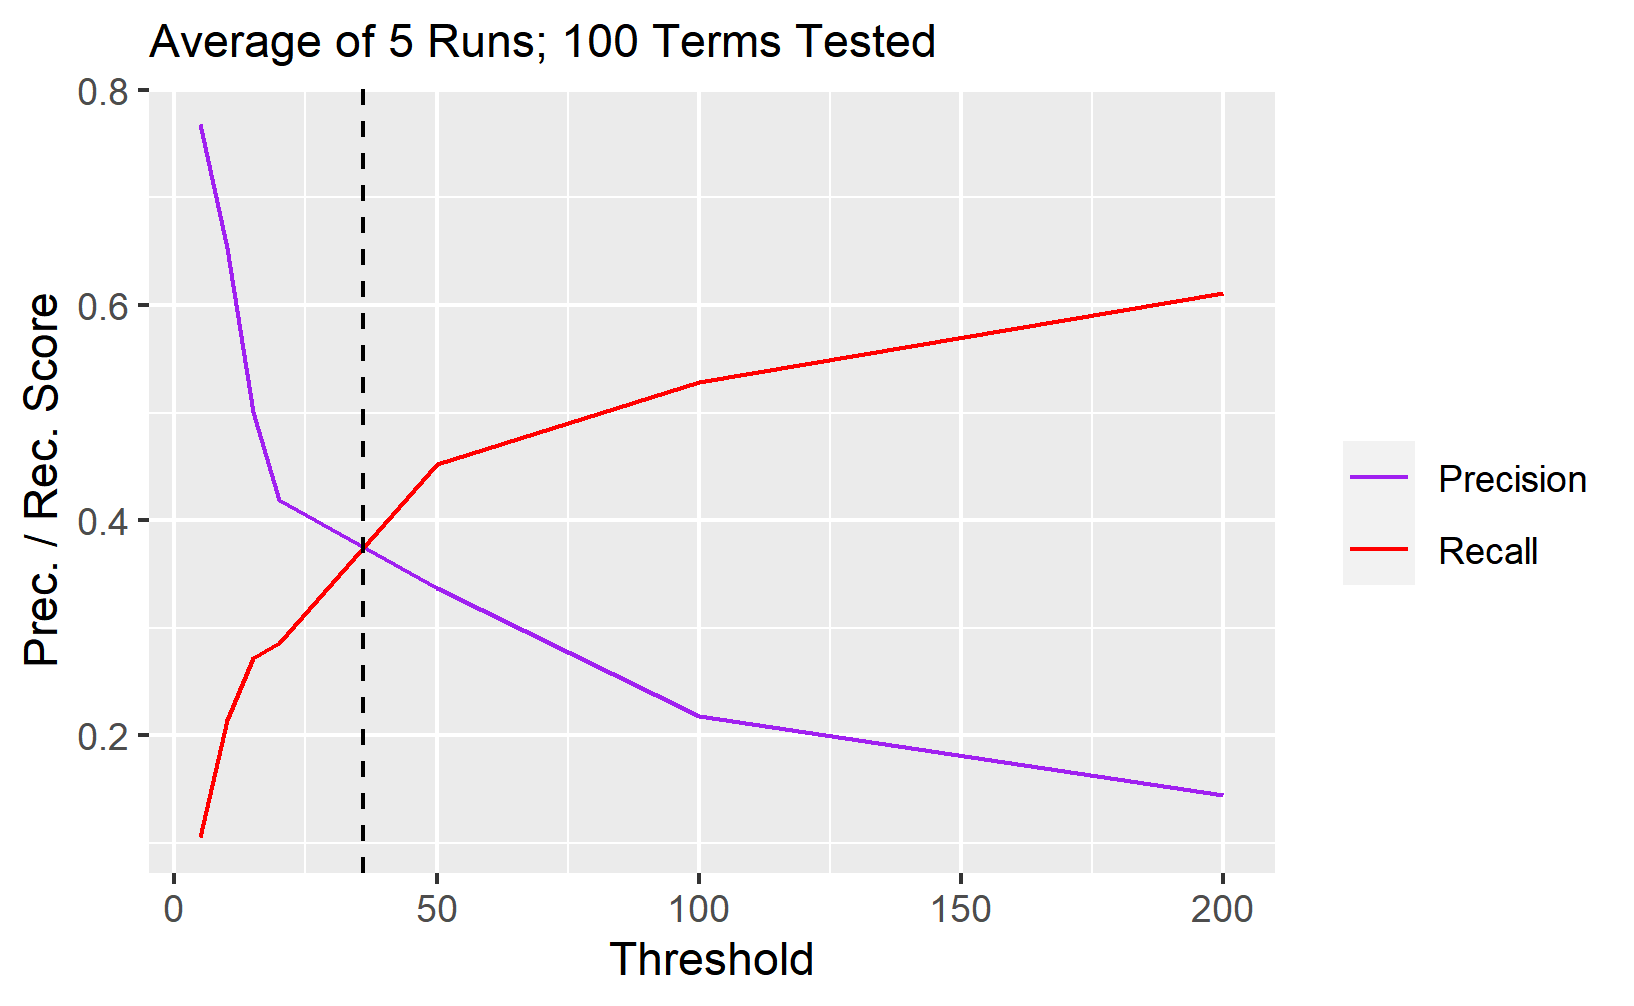
\includegraphics[width=\linewidth]{figs/precision_recall.png}
        \caption{Precision Recall results}
    \end{center}
    \label{fig:evaluation}
\end{figure}


As can be seen in the figure \ref{fig:evaluation}, the optimal value for precision and recall would be 36 most frequent terms, for our data.
Generally, it can be said that there is a trade-off between quality of expert recommendation and the quantity.
If an increase in precision is requested, lower threshold values are sensible to increase the quality of results.
It must also be noted, with 36 terms à 6 authors, we have 216 automatically determined terms. 
Thus, here our manually determined keywords only make-up around 44 \% (170 terms), and not the majority as would be expected in a bad system for the intersection of precision and recall.


\section{Conclusion} % Critical look at our work
Summarizing our findings.

Answer each individual research question.

What could future projects improve on?

What can we improve upon?

What is the main take-away?

...

...

\section{References}

\bibliography{references}
\bibliographystyle{plain}

\end{document}
